\documentclass{article}
\usepackage{amsmath}
\usepackage{graphicx}
\usepackage{float}
\usepackage[style=authoryear-ibid,backend=biber]{biblatex}
\title{SIRD Model over Small World, Scale Free Graphs}
\date{08/02/2023}
\author{Thomas Draycott}
\addbibresource{references.bib}
\graphicspath{ {./images/} }
\begin{document}
    \maketitle
    \pagenumbering{arabic}
    \newpage
    \tableofcontents
    \newpage
    \section{Introduction}
    This project seeks to investigate the structural differences between random graphs and small-world, scale-free graphs and Albert-Barabási graphs. Then, these properties will be tested by how they affect an SIRD model ran on both types of graph. The motivation for this project was from a deep interest in graph theory and with the recent COVID-19 pandemic how the ways human relations may affect the spread of infectious disease.
    


    \section{Literature Review}
        \subsection{Graph Theory}
        Graph Theory is the study of networks where vertices are connected by edges, see APPENDIX for a further explanation.
        \subsection{Random Graphs}
        TO DO
        \subsection{Small World Graphs}
        In May 1967 Professor of Psychology at the Graduate School and University Center of the City University of New York, Stanley Milgram ran an experiment to see if a person living
        in Omaha, Nebraska could get a parcel to a stockbroker in Boston, Massachusetts \parencite{milgram1967small}. In his experiment he found the average path length to reach the stockbroker was 5.5, which created the term
        six degrees of separation (however Milgram's experiment had flaws which puts the exact number into doubt). This idea of having such a small average path length for such numerous nodes is a hallmark of a small world graph.\\
        A Small world graph is formally defined by the following property: $L\propto\log{N}$ where $L$ is the average shortest path length of the network and $N$ is the total number of nodes \parencite{Watts1998}. Several models exist to generate small world graphs such as the Watts-Strogatz Model.

        \subsection{Scale Free Graphs}
        In networks that appear in the real world such as the internet and social groups, there exists nodes known as "hubs" (a node that has a higher degree then the average of the graph). This is an important property encapsulated in Scale-Free Graphs.\\ 
        Scale-free Graphs are formally defined by the following power law: $P(k) \sim  k^{-\gamma }$, $k$ is the degree of a vertex, $P(k)$ is the probability of a node having degree $k$ and $\gamma$ is a parameter determined by the graph typically $2<\gamma<3$ \parencite{onnela2007structure}.

        \subsection{Barabasi-Albert Model}
        In 1999, Albert-László Barabási and Réka Albert developed the Albert-Barabási Model which generates small world, scale free graphs by a process of preferential attachment \parencite{barabasi1999emergence}. The model works as such: define two parameters $n$ (The number nodes the graph at the end of the process will have) and $e$ (the number of edges added for each new node) take a seed graph, add one new node to the graph, using preferential attachment add $e$ edges from the new node to nodes on the seed graph, continue till there are $n$ nodes on the graph.\\
        Preferential attachment describes a 'rich get richer effect' that is the higher the degree of the node the more likely it will gain a new edge, the following formula describes it $\prod (k_{i}) = \frac{k_{i}}{\sum_{j} {k_{j}}}$ where $k_{i}$ is the degree of node $i$. 
        \subsection{SIRD Model}
        SIRD stands for Susceptible, Infected, Recovered and Dead which is the states each individual in the model can take. There are many was of implementing a model like this such as a virus having specific infection 'power' and mortality rates or having the infection be determined entirely by the individual.
    \section{Mathematical Methods}
        \subsection{Python}
        This project is written in the Python programming language as it is the language I am most familiar with and has very useful modules for graph analysis. All the code to create these graphs is completely doable without 3rd party libraries however as this project focuses on more complicated topics than just graph creation I will be using a 3rd party library to simplify creating graphs and manipulating them as detailed below.
        \subsection{Networkx}
        To begin we should explain the software that this project is based most heavily on. Networkx is a module for the Python programming language that allows for the creation and manipulation of graphs \parencite{SciPyProceedings_11}.
        \subsection{Creating Graphs}
        First we need to show how to create a graph using the software.\\
        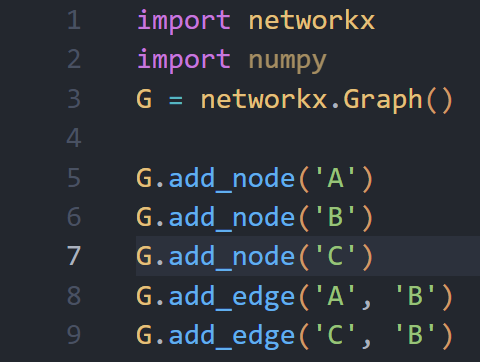
\includegraphics[width=8cm]{images/add_nodes_add_edges.png}\\
        The above code does the following: it imports the Networkx package for us to use, creates a 'graph' object called G, creates nodes A, B, C, then adds two edges between A and B and B and C.\\
        However that is too clunky for normal use so the Networkx package provides functions such as:
        \begin{verbatim}networkx.complete_graph(5)\end{verbatim}
        to generate a complete graph with 5 nodes in one line, but we still have the atomic control of the graph as in the first example.
        \subsection{Creating Random Graphs}
        To create a random graph on a piece of paper it is quite simple: Select $N$ nodes to add to the graph and $p$ probability, draw $N$ nodes on the paper, then go through every possible pair of nodes in the graph and draw an edge between them if when picking a random real number from [0,1] it is less than $p$. Networkx implements a function \verb|networkx.gnp_random_graph| to create a random graph using the following code:
        \begin{figure}[H]
            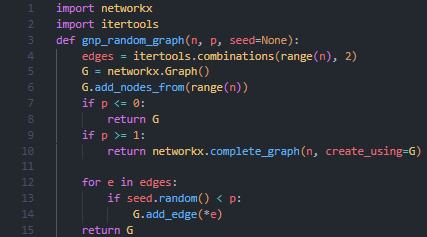
\includegraphics[width=8cm]{images/CreatingRandomGraphs.png}
            \caption{The Random Graph Function}
            \label{fig:RandomGraph1}
        \end{figure}
        Let's explain, the function takes $n$ (The total number of nodes) and $p$ (The probability of drawing an edge between a pair of nodes) as parameters. The \verb|itertools.combinations(range(n),2)| creates s list of every combination of 2 numbers up to $n$ i.e. (0,1), (0,2), (1,2) and so on, then to graph $G$ we add $n$ nodes, if $p = 0$ then there are 0 edges in the graph, so it stays empty and if $p =1$ then every node is attached to every other node, so it becomes a complete graph, if neither of those are true then we loop through all the possible combinations of nodes and choose a random number from $[0,1]$ and if that is less than $p$ we add an edge between those nodes.
        \subsection{Creating Barabasi-Albert Graphs}
        First let us describe how to create Barabasi-Albert Graphs on a piece of paper. To create a Barabasi-Albert Graph we must first start with a "seed" graph (An already drawn graph that we will grow using the Barabasi-Albert Model) then we will define two more parameters $n$ for the total number of nodes we want this new graph to have and $m$ the number of edges we will add each iteration of the model. The algorithm works in the following way: take your "seed" graph and assign each node on the graph a probability $p$ according to its degree $k$ using the formula $p(k_{i}) = \frac{k_{i}}{\sum_{j} {k_{j}}}$ we then randomly select $m$ unique nodes according to the probabilities calculated (this can be done by label each node 1 to n then write on a piece of paper that label for each node, then fold the paper a number of times proportional to its probability for example folding 0.2 twice but 0.2 five times then randomly choosing the papers), add 1 new node to the graph and draw and edge from this new node to each of the randomly preexisting nodes, repeat this until we have $n$ nodes on the graph.
        As Barabasi-Albert graphs are the main focus of this project we will now show how they are created in networkx. 
        \begin{figure}[H]
            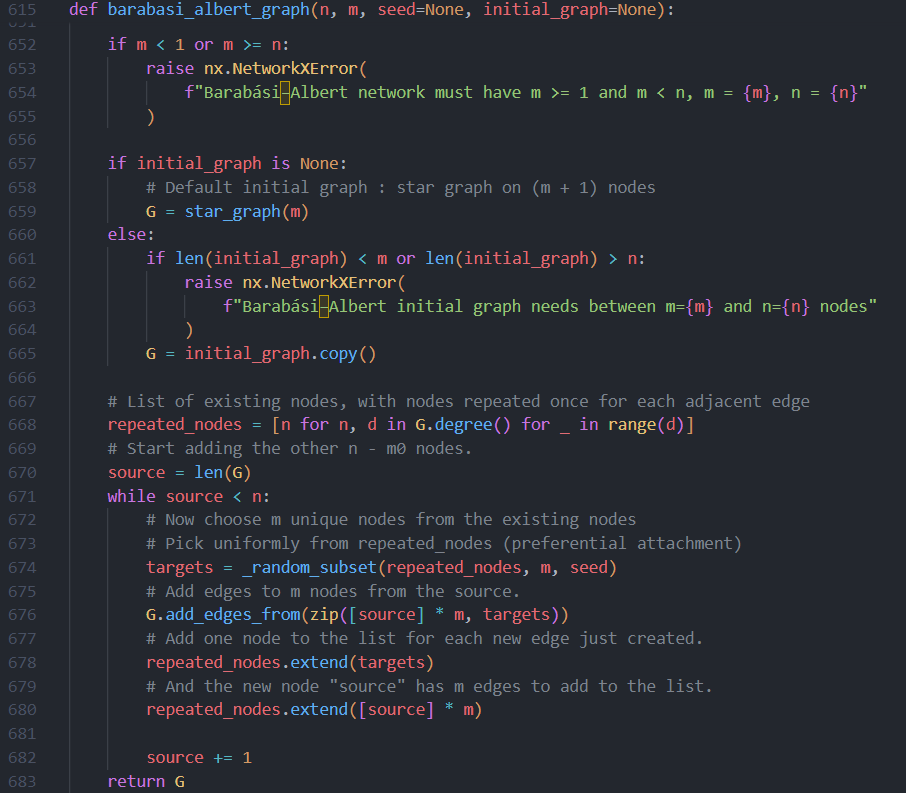
\includegraphics[width=8cm]{images/BARABASI_FUNC.png}
            \caption{The Barabasi-Albert Graph Function}
            \label{fig:Barabasi-Albert function1}
        \end{figure}

        TO DO
        \subsection{Gaining Information From Graphs}


    \section{Analysis}
    TODO
    \section{Evaluation}
    TODO
    \section{APPENDIX}
        \subsection{Python Code}
        ADD CODE HERE
        
    
    
\printbibliography
\end{document}